\chapter{Sistema de Recomendação de Rotas de Pontos Turísticos Baseado em Filtragem Colaborativa}
\label{chp:eTourismRecSys}

Para que um software seja desenvolvido de forma consistente, é necessário aliar boas práticas da engenharia de software com um robusto e eficiente processo de desenvolvimento. Neste capítulo, é mostrada as ferramentas utilizadas neste projeto, discutindo seus objetivos e funcionalidades no sistema.
% Um processo de software é um conjunto de atividades que leva ao desenvolvimento do produto. O processo define quem faz, o que faz e quando fazer mas nem sempre diz como fazer. O desenvolvedor ou a organização desenvolve seus próprios processos, significando que não existe um processo ideal \citep{Sommerville2010}. 

\section{Requisitos}
\label{sec:requirements}

% Os requisitos de software são detalhes do que o sistema realizará, os serviços que fornece e as restrições em sua operação \citep{Sommerville2010}. 
O objetivo dessa fase é reunir informações sobre o problema a ser resolvido, de acordo com o que é proposto nesse trabalho. Nessa seção, são detalhados os requisitos do sistema desenvolvido como proposta deste trabalho, fornecendo informações necessárias para o projeto e implementação. Os requisitos de software são classificados como requisitos funcionais e requisitos não funcionais.

% \begin{enumerate}
%     \item \textbf{Requisitos funcionais}: descrevem explicitamente as funcionalidades e os serviços do sistema. Documenta como o sistema deve reagir a entradas específicas, como deve se comportar em determinadas situações e o que o sistema não deve fazer \citep{Sommerville2010}.
%     \item \textbf{Requisitos não funcionais}: definem propriedades e restrições do sistema, podem ser do todo ou parte do sistema. Este tipo de requisito pode ser mais crítico que os requisitos funcionais:se não satisfaz, o sistema é inútil \citep{Sommerville2010}. 
% \end{enumerate}

\subsection{Requisitos Funcionais e Não Funcionais}
\label{subsec:functional_requirements}

Na identificação dos requisitos, foram utilizadas as seguintes convenções: [FRXX] para requisitos funcionais e [NFRXX] para os requisitos não funcionais. São dadas prioridades aos requisitos, que servem para indicar a relevância do requisito para o sistema proposto. Essas são classificadas em: 

\begin{enumerate}
    \item \textbf{Básica}: são requisitos que devem ser implementados. Caso não sejam realizados, o sistema não pode funcionar ou não atende o objetivo da proposta.
    \item \textbf{Significativo}: são requisitos que o sistema pode funcionar, porém de forma parcial.
    \item \textbf{Relevante}: estes requisitos não comprometem o funcionamento básico do sistema; podem ser deixados para versões posteriores deste trabalho.
\end{enumerate}

A Tabela \ref{tab:functional_requirements} apresenta os requisitos funcionais do sistema e a Tabela \ref{tab:non-functional_requirement} apresenta os requisitos não funcionais do sistema, classificados por suas características.

\begin{table}[H]
    \centering
    \begin{tabular}{|c|p{4.5cm}|p{6.5cm}|c|}
        \hline
		
		\multicolumn{1}{|c|}{\bfseries Código} & \multicolumn{1}{c|}{\bfseries Nome} & \multicolumn{1}{c|}{\bfseries Descrição} & \multicolumn{1}{c|}{\bfseries Prioridade} \\ \hline
		
        FR01 & Realizar recomendações de pontos turísticos & Mostrar sugestões de locais para visitação & Básica \\ \hline
        FR02 & Gerar rotas para o usuário & Gerar rotas de acordo com os pontos recomendados pelo sistema, considerando origem e destino do usuário & Básica \\ \hline
        FR03 & Realizar pontos turísticos com base nas informações do usuário & De acordo com as preferências prévias do usuário de outros pontos de localização, gerar recomendações de pontos de acordo com as informações do usuário & Significativo \\ \hline
        FR04 & Gerar a rota com a menor distância para o usuário & Com os resultados obtidos no sistema de recomendação, gerar a menor rota para o usuário & Relevante \\ \hline
        FR05 & Gerar a rota com a menor distância e a maior quantidade de pontos para o usuário & Fornecer ao turista uma rota com a menor distância e com a maior quantidade de pontos de interesses, de acordo com resultados do sistema de recomendação & Relevante\\ \hline
        FR06 & Realizar recomendações, considerando os pontos de origem e destino do usuário & De acordo com a localização do usuário e o destino final da sua rota, considerar o atributo distância na recomendação de pontos & Relevante \\ \hline
    \end{tabular}
    \caption{Requisitos Funcionais do Sistema.}
    \label{tab:functional_requirements}
\end{table}

\begin{table}[H]
    \centering
    \begin{tabular}{|c|p{8.3cm}|c|c|}
        \hline
		
		\multicolumn{1}{|c|}{\bfseries Código} & \multicolumn{1}{c|}{\bfseries Descrição} & \multicolumn{1}{c|}{\bfseries Característica} & \multicolumn{1}{c|}{\bfseries Prioridade}
		\\ \hline
		
        NFR01 & O sistema deve mostrar a rota gerada de uma forma fácil e simples de usar, sem a necessidade de manuais ou treinamento & Usabilidade & Básica \\ \hline
        NFR02 & O sistema deve recomendar pontos turísticos com veracidade & Corretude & Significativo \\ \hline
        NFR03 & O sistema deve gerar rotas seguras dos pontos turísticos recomendados & Corretude & Significativo \\ \hline
        NFR04 & O sistema deve recomendar os pontos turísticos e gerar a rota de uma maneira rápida & Eficiência & Significativo \\ \hline
    \end{tabular}
    \caption{Requisitos Não Funcionais do Sistema.}
    \label{tab:non-functional_requirement}
\end{table}

\section{Arquitetura}
\label{sec:architecture}

Conforme \cite{Bass:2012:SAP:2392670}, arquitetura de software de um programa ou sistema operacional é a estrutura ou estruturas do sistema, que abrange os componentes de software, as propriedades externamente visíveis desses componentes e as relações entre eles.

% Neste projeto, a aplicação foi desenvolvida utilizando o padrão \textit{pipe and filter} (duto e filtro, em português), onde é um modelo no qual as transformações funcionais processam suas entradas e produzem saídas \citep{Sommerville2010}. Neste padrão, o processamento dos dados em um sistema está organizado de modo que cada componente de processamento, chamado filtro, seja discreto. Os dados fluem (como em um duto) de um componente para outro para processamento \citep{Sommerville2010}. 

A Figura \ref{fig:Tourisys_pipe_filter} mostra a arquitetura \textit{pipe and filter} (duto e filtro, em português) para este trabalho. Cada componente (na figura, representados pelos quadrados) age como filtro, realizando as validações dos conteúdos obtidos, transformações e processamentos de dados. Entre um filtro e outro, existem os canais, que agem como dutos.

\begin{figure}[H]
    \centering
    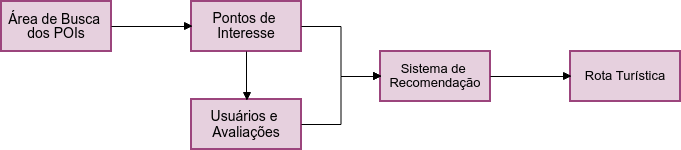
\includegraphics[width=\textwidth]{images/Tourisys_Pipe_Filter.png}
    \caption{Arquitetura do projeto}
    \label{fig:Tourisys_pipe_filter}
\end{figure}

\section{Tecnologias}
\label{sec:technologies}

Para o desenvolvimento do sistema foram utilizadas diversas tecnologias: linguagens de programação, \textit{frameworks}, entre outras. A seguir são apresentadas essas tecnologias.

\subsection{HTML/CSS/JavaScript}

HTML\footnote{https://www.w3.org/html} é uma linguagem de marcação padrão para criar páginas Web. Sua sigla vem do inglês, que significa \textit{HyperText Markup Language}, que significa Linguagem de Marcação de Hipertexto. O HTML é uma linguagem para publicação de conteúdo (texto, imagem, vídeo, áudio etc.) na Web \citep{w3cHTML}. Ela foi utilizada para construir as páginas com as rotas dos pontos turísticos recomendados, que possibilitam a interação do usuário com o sistema.

\textit{Cascading Style Sheets}, mais conhecido como CSS\footnote{https://developer.mozilla.org/en-US/docs/Web/CSS} é uma linguagem de estilo utilizada para descrever a apresentação de um documento escrito em HTML e como os elementos devem ser renderizadas na tela ou em outros meios de comunicação. A tecnologia \textit{JavaScript} (JS)\footnote{https://developer.mozilla.org/bm/docs/Web/JavaScript} é uma linguagem de programação interpretada. Muito conhecida como uma linguagem voltada para páginas Web, a utilização de JS está sendo expandida para outros ambientes. Por exemplo, desenvolvimento de jogos, interfaces para sistemas operacionais, aplicações mobile, banco de dados, entre outros.

\subsection{Python/GraphLab}

Python\footnote{https://www.python.org/} é uma linguagem de programação interpretada, interativa e orientada a objetos. Foi lançada em 1991 por Guido van Rossum. Está disponível para as mais diversas plataformas, incluindo consoles de jogos eletrônicos ou alguns celulares. Caso o sistema operacional não suporte, é possível compilar a partir do código fonte através de um compilador C. Ao longo do tempo, vem sendo desenvolvidas muitas bibliotecas de funções especializadas que permitem expandir as capacidades base da linguagem.
Uma das bibliotecas utilizadas neste trabalho é a GraphLab Create\footnote{https://turi.com/}. É um pacote que permite realizar análise de dados em larga escala. Inclui diversas ferramentas para o desenvolvimento de modelos preditivos de aprendizagem de máquinas e sistemas de recomendação, além da exploração e a visualização de dados.

\subsection{OpenStreetMap/Overpass API}

OpenStreetMap\footnote{http://www.openstreetmap.org} é projeto de produção colaborativa de dados geo-espaciais abertos. Qualquer pessoa pode contribuir e editar o mapa, mantendo atualizadas as informações sobre estradas, pontos de interesses, trilhas, meios de transportes, entre outros, ao redor do mundo. Utilizando informações do OpenStreetMap, o Overpass API\footnote{http://overpass-api.de/} é um serviço que é possível obter informações personalizadas dos dados do mapa do OpenStreetMap. Através dessa ferramenta são obtidos os pontos de interesses relacionado ao turismo com as suas respectivas informações, como nome, descrição, horário de funcionamento, latitude e longitude. Atua como um banco de dados na Web: o cliente envia uma consulta para a API e tem como resultado o conjunto de dados que corresponde à consulta.

\subsection{Google Maps API}

A API\footnote{https://developers.google.com/maps/} do Google Maps é uma plataforma que permite criação de mapas de diferentes tipos (satélite, terreno, entre outros) e com locais definidos, controle de zoom, geração de rotas, pesquisa por estabelecimentos, e outras coisas.
Em nossa pesquisa, essa ferramenta é utilizada para obter informações atualizadas sobre os pontos de localização que estão cadastrados na plataforma, além das avaliações dos usuários do local específico (Google Places API\footnote{https://developers.google.com/places/web-service/}).

\section{Funcionamento}
\label{sec:operation}

A princípio utiliza-se informações dos pontos de interesses obtidos através do OpenStreetMap. Com base nessas informações, são obtidas as avaliações dos usuários que estão registradas no Google Maps. A Figura \ref{fig:tourisys_operation} mostra um fluxograma com uma visão geral do funcionamento do sistema.

Inicialmente (passo 1 da Figura), é definido a região de pesquisa dos pontos turísticos. Para isso, é necessário inserir duas localizações (duas latitudes e duas longitudes) que delimitam a área de busca, que forma-se um quadrado chamado \textit{bounding box} (em português, caixa delimitadora). Depois, no passo 2, o sistema irá obter as informações dos pontos de interesse (que no sistema de recomendação serão tratados como itens) de acordo com as categorias dos pontos turísticos:

\begin{multicols}{2}
    \begin{itemize}
        \itemsep0em
        \item Centros de Arte
        \item Obras de Arte
        \item Atrações
        \item Casino
        \item Castelos
        \item Galerias
        \item Patrimônios
        \item Locais Históricos
        \item Centros de Informações
        \item Monumentos e Memoriais
        \item Árvore Monumental
        \item Museus
        \item Locais de Piquenique
        \item Estátuas
        \item Parques temáticos
        \item Panoramas
        \item Vinhedos
        \item Moinhos
        \item Zoológico
    \end{itemize}
\end{multicols}

Cada item tem os atributos: (1) ID do local cadastrado no OpenStreetMap; (2) Nome do ponto turístico; (3) Tipo (categoria) do local; Localização do ponto de turístico, que é composto de: (4) Latitude do ponto turístico; e (5) Longitude do ponto turístico. A base de dados somente contém locais que estão inseridos nessas categorias e os itens podem ter mais de uma categoria.

Com esses resultados, segue-se para o passo 3, no qual coleta-se os dados dos usuários que deixaram suas avaliações nos locais obtidos no passo 1, através da API do Google Maps. Para obter as notas e quais são os usuários, é necessário ID do local registrado no Google Maps. Por isso, são necessárias duas requisições: uma para buscar o ID do ponto de interesse (conhecido como \textit{place ID}) e uma outra requisição para consultar as análises dos pontos. Na primeira requisição, os parâmetros necessários são as informações da latitude e longitude do local e o nome. Na segunda requisição, basta o \textit{place ID} obtido na consulta anterior.

Essas informações são inseridas em duas bases de dados: a que contém as avaliações e outra que contém atributos do usuário. A base de avaliações compreende de: (1) ID do local cadastrado no OpenSteetMap; (2) ID do usuário que realizou a avaliação; (3) Nota dada pelo usuário no ponto turístico; (4) Data e hora da avaliação do usuário no formato \textit{timestamp}. A base de usuários é composta de (1) ID do usuário cadastrado no Google Maps; (2) Nome do usuário.

\begin{figure}[H]
    \centering
    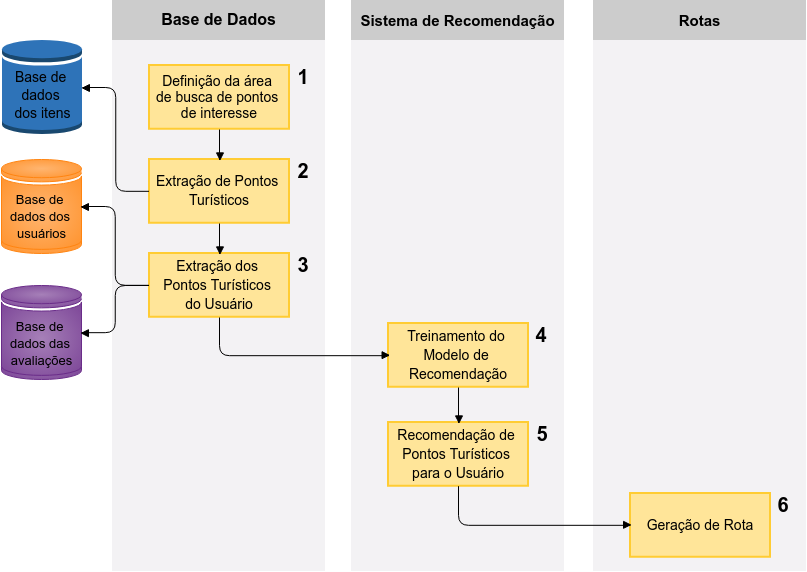
\includegraphics[width=\textwidth]{images/Tourisys_Funcionamento.png}
    \caption{Fluxo do Funcionamento do Sistema.}
    \label{fig:tourisys_operation}
\end{figure}

Diante da base de dados pronta, passa para o passo 4, para o treinamento do modelo do sistema de recomendação. Nessa fase, o sistema está pronto para recomendar pontos turísticos não só para novos usuários mas para também usuários que estão contidos na base de dados formada no passo anterior. No passo 5 é realizada a recomendação de pontos turísticos para o usuário. De acordo com o modelo de recomendação escolhido, o usuário informa pelo menos um local que já tenha visitado e que este esteja contido na base de dados do sistema. Com essas informações, é possível gerar recomendação para aquele determinado usuário com locais que possam ser do interesse do turista.

O último passo é a geração do mapa. É gerada uma página HTML, que mostra a rota que deve ser feita para a visitação dos pontos turísticos, de acordo com o gosto do usuário. Esse mapa é construído através da API do Google Maps, no qual é informado o local de origem e destino e os pontos de parada, que são os pontos do resultado do passo anterior.

\section{Modelo de Usuário}

Para construir o modelo de usuário, é preciso detectar e somar todas as informações básicas do perfil. O modelo de usuário deste projeto segue a metodologia de \cite{Brusilovsky:2001:AH:598284.598341}, incorporando as atividades do usuário. 

Neste trabalho, a princípio, é analisado uma única informação monitorada, favorável para a utilização, que são os conjuntos dos pontos turísticos já visitados pelo usuário. Este conjunto é um forte indicador do interesse do usuário, pois apresenta qual a vontade do turista através da categoria dos locais. Desse modo, este projeto se assemelha muitos com sistemas de recomendação baseados na experiência do usuário, como é apresentado na seção \ref{subsec:eTourism_recsys_userXP}.

A localização de origem e destino do usuário é uma grande utilidade na recomendação de pontos turísticos. Através dessas informações, pode-se sugerir locais turísticos próximos desses pontos. Por enquanto, é necessário o usuário inserir manualmente os pontos de início e fim da rota. Nos trabalhos futuros, essa recomendação poderá ser feita em tempo real, monitorando a localização atual do usuário e sugerindo não só os pontos de interesse, mas também pontos finais da rota. Além disso, pode-se considerar outros pontos turísticos que o usuário visitou através do histórico de localização.

\section{Modelo de Pontos de Interesse}

No nosso contexto, são utilizados para testes dois tipos de modelos de itens, ou pontos de interesse: o modelo baseado em similaridade, através do algoritmo \textit{Item Similarity}; e o modelo baseado em conteúdo, com o algoritmo \textit{Item Content}. Cada modelo trabalha de formas diferentes.

\subsection{Modelo de Pontos de Interesse Baseado em Similaridade}

No modelo de pontos de interesse baseado em similaridade, é necessário calcular a similaridade entre os itens usando as observações dos usuários que interagiram com dois ou mais itens. Dado uma similaridade entre os itens $i$ e $j$, $S(i,j)$ classifica um item $j$ para o usuário $u$ usando uma média ponderada das observações anteriores do usuário $I_u$ \citep{Ricci:2010:RSH:1941884}. Para este modelo utiliza-se o algoritmo \textit{Item Similarity}, que usa as semelhanças de item por item baseado nos usuários em comum para criar a recomendação. Existem diversas métricas de similaridade: \textit{Jaccard}, \textit{Cosine} e \textit{Pearson Correlation}.

\subsubsection{Métricas de Similaridade}
\label{subsubsec:similarity_metrics}

A similaridade \textit{Jaccard} é utilizada para medir a similaridade entre dois conjuntos de elementos \citep{Ricci:2010:RSH:1941884}. No contexto de recomendação, a similaridade \textit{Jaccard} entre dois itens é calculada da seguinte forma:

\begin{equation}
    \mbox{JS}(i,j) = \frac{|U_i \cap U_j|}{|U_i \cup U_j|}
\end{equation}

no qual $U_i$ é o conjuntos de usuários que avaliaram o item $i$. Jaccard é uma boa escolha quando somente contém avaliações implícitas dos itens (exemplo: pessoas avaliaram ou não) ou quando a informação de quantas estrelas o item recebeu não é significativo. Se é necessário a comparação entre as avaliações dos itens, as similaridades \textit{Cosine} e \textit{Pearson Correlation} são recomendadas \citep{Ricci:2010:RSH:1941884}.

A similaridade \textit{Cosine} entre dois itens é calculada da seguinte forma:

\begin{equation}
    \mbox{CS}(i,j) = \frac{\sum_{u\in U_{ij}} r_{ui}r_{uj}}
    {\sqrt{\sum_{u\in U_{i}} r_{ui}^2} \sqrt{\sum_{u\in U_{j}} r_{uj}^2}}
\end{equation}

no qual $U_i$ é o conjuntos de usuários que avaliaram o item $i$ e $U_ij$ é o conjunto de usuários que avaliaram tanto o item $i$, tanto o item $j$. Um dos problemas da similaridade \textit{Cosine} é que ela não considera as diferenças entre a média e a variância das avaliações feitas para os itens $i$ e $j$ \citep{Ricci:2010:RSH:1941884}. Para resolver este problema, a similaridade \textit{Pearson Correlation} compara avaliações, removendo os efeitos das médias e das variâncias. Calcula-se esse coeficiente segundo a fórmula:

\begin{equation}
    \mbox{PS}(i,j) = \frac{\sum_{u\in U_{ij}} (r_{ui} - \bar{r}_i)(r_{uj} - \bar{r}_j)}
    {\sqrt{\sum_{u\in U_{ij}} (r_{ui} - \bar{r}_i)^2} \sqrt{\sum_{u\in U_{ij}} (r_{uj} - \bar{r}_j)^2}}
\end{equation}

em que $U_ij$ é o conjunto de usuários que avaliaram os itens $i$ e $j$; $r_ui$ é a avaliação que o usuário $u$ deu ao item $i$; $r_uj$ é a avaliação que o usuário $u$ deu ao item $j$, $\bar{r}_i$ é a media das avaliações do item $i$ e $\bar{r}_j$ é a media das avaliações do item $j$.

\subsection{Modelo de Pontos de Interesse Baseado em Conteúdo}

No modelo de pontos de interesse baseado em conteúdo, o índice de similaridade entre dois itens é calculado pela primeira vez que mede a similaridade entre os dados do item para cada coluna. Em seguida, é medida a média ponderada das similaridades por coluna, para obter a semelhança final. As recomendações são geradas de acordo com a similaridade média de um item candidato com todos os itens no conjunto de itens classificados de um usuário.

Nesse cenário, as informações relevantes que são consideradas são as categorias e a localização. A categoria diz respeito ao que é o ponto turístico, caracterizando-o de acordo com o que o local oferece ao turista. A localização fornece informações específicas de latitude e longitude do local. Todas as duas informações são pré-definidas e não precisam da interação do usuário. Formalmente, o modelo de pontos de interesse baseado em conteúdo é um par $(C,L)$:

\begin{itemize}
    \item $C$ representa o conjunto de categorias do ponto turístico. As categorias são pré-definidas e estáticas enquanto não houver uma atualização no sistema do OpenStreetMap\footnote{https://www.openstreetmap.org/} que as modifique. Cada elemento do conjunto de categorias tem a mesma importância para este modelo.
    \item $L$ representa a localização do ponto turístico. As localizações são pré-definidas e estáticas. Especificamente, a localização é composta da latitude e longitude do local.
\end{itemize}

Outras informações sobre o ponto de interesse em si, como nome, também podem ser úteis. Para melhor entendimento, o seguinte exemplo mostra o modelo de um ponto turístico:

\begin{itemize}
    \item $C = \{"arts\_centre", "attraction"\}$ representam as categorias da loja, indicando que é um local de centro de artes e uma atração;
    \item $L$ = (-12.9995737,-38.5296316), que representa a latitude e longitude do ponto turístico, respectivamente.
\end{itemize}

\section{Sumário}

Neste capítulo, mostra-se uma visão geral sobre os aspectos do desenvolvimento do sistema. Discutiu-se sobre a arquitetura do sistema, abordando os aspectos da estrutura do sistema. Foram apresentadas as ferramentas e tecnologias utilizadas e como é o funcionamento do sistema construído. No próximo capítulo \ref{chp:evaluation} será realizada uma avaliação do trabalho realizado, discutidas metodologia, métricas de avaliação e os resultados obtidos.